\chapter{Fundamentos}
\label{chap:fund}
Neste capítulo introduzimos alguns conceitos sobre inteligência artificial com o objetivo de apresentar ao leitor conceitos que serão utilizados em seções futuras.

\section{Processo de Decisão de Markov}
\label{ssec:mdp}

Processos de Decisão de Markov (em inglês, \textit{Markov Decision Process}, ou \textbf{MDP})
são uma forma de representar alguns problemas de decisão sequenciais.

\begin{figure}[!ht]
    \centering
    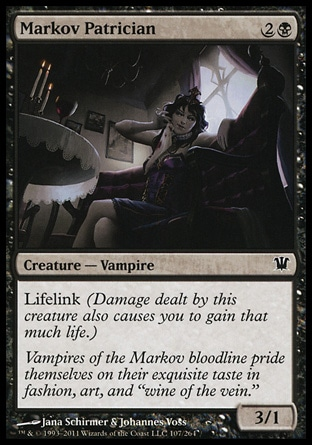
\includegraphics[width=0.3\textwidth]{picstcc/markov.jpg}
    \caption{Na história do jogo, Markov é um poderoso clã de vampiros.}
    \label{markovcard}
\end{figure}
\vskip1ex
Para descrever um MDP, usaremos um exemplo com o intuito de tornar a explicação mais didática.
Imagine que um gerente de um galpão de um produto tem como objetivo maximizar o lucro esperado
para o próximo ano. A cada mês, o gerente observa quanto há em estoque do produto e decide
quanto irá pedir ao distribuir para o próximo mês. A demanda mensal do produto é desconhecida,
mas segue uma distribuição de probabilidade conhecida. Se o gerente pedir produto demais, terá
custos para manter o estoque, e se pedir de menos, estará perdendo vendas por falta de inventário.
Suponha que o galpão tem capacidade para armazenar $M$ unidades de produto e que os custos e a
distribuição da demanda não muda de mês para mês.
\vskip1ex
O primeiro conceito de MDP que iremos introduzir é o de \textbf{época de decisão}. Uma época de
decisão é um momento onde uma decisão é tomada. No nosso exemplo, cada época de decisão ocorre
no começo de um mês, quando o gerente deve decidir quanto produto irá pedir ao distribuidor. Chamamos
a quantidade de épocas de decisão de um MDP de \textbf{horizonte}, que pode ser finito ou infinito.
No exemplo, o horizonte é finito de tamanho $12$, sendo uma época para cada mês do ano no qual o
gerente deseja maximizar seus lucros.
\vskip1ex
Um MDP pode ser representado por uma tupla $(S, A, P, R)$. $S$ é o conjunto de \textbf{estados}
$s_t$ do problema, onde um estado é uma configuração do problema em uma determinada época de
decisão $t$. No exemplo, cada estado representa o espaço disponível no galpão, que pode variar
de $0$ a $M$.
\vskip1ex
$A$ é o conjunto de \textbf{ações} $a_t$, onde $t$ é a época de decisão. No exemplo, uma ação
pode ser comprar de $0$ a $M-s_t$ unidades no mês.
\vskip1ex
Para falar sobre os outros elementos da tupla do MDP, precisamos entrar em detalhes sobre os
custos para pedir o produto ao distribuidor e manter o produto em estoque. Um mês começa com $s_t$
unidades em estoque, e são encomendadas mais $a_t$ unidades, o que gera um custo $c_{pedido}$ dado
pela função $c_p(a_t)$. Vamos assumir que as unidades sejam pedidas no começo do mês e sejam vendidas
no final do mês. Há, portanto, um custo $c_{estoque}$ para manter o produto em estoque dado pela função
$c_e(s_t + a_t)$. A probabilidade de que a demanda $D_t$ no mês seja de $j$ unidades é $p_j, j = 0,1,2\ldots$.
Quando o final do mês chegar, o número de unidade vendidas será $x_t = min{D_t, s_t + a_j}$, e o lucro
será dado pela função $l(x_t)$. O número de unidades que começarão o próximo mês em estoque será
$s_{t+1}= s_t + a_t - x_t$.
\vskip1ex
$R: S \times A \mapsto \mathbb{R}$ é a função que dá a \textbf{recompensa} esperada por tomar a ação $a_t$
quando o processo está no estado estado $s_t$. No exemplo, $r_t(s_t, a_t) = E[l(x_t)] - c_{estoque} - c_{pedido}$.
\vskip1ex
$P: S \times A \times S \mapsto [0,1]$ é uma função que dá a \textbf{probabilidade} do sistema passar de um estado
para outro, dado uma determinada ação. No nosso exemplo:

\begin{equation*}
  Pr\{s_{t+1} = j|s_t = s, a_t = a\} = \begin{cases}p_{s+a-j}, &j\le s + a \\
                                                    \sum\limits_{i=s+a}^\infty p_i, &j=0 \\
                                                    0, & j >s+a\end{cases}
\end{equation*}

Uma vez que temos o nosso MDP definido, queremos chegar em uma \textbf{política}, que é o nome dado
ao conjunto das \textbf{regras de decisão}. Uma regra de decisão $d_t(s)$ é uma função $d: S \mapsto A$
que que, dado um estado $s$ na época de decisão $t$, retorna uma ação $a$ que deve ser tomada a partir
daquele estado de modo a maximizar o ganho final.

\section{Busca em grafo}
\label{sec:search}
Podemos representar um problema de Inteligência Artificial como um grafo.\footnote{Neste texto, sempre que mencionarmos \textit{grafos} estaremos nos referindo \textit{grafos dirigidos}.} Um grafo $G$, resumidamente, é um conjunto $G = (V, E)$, onde $V$ é chamado conjunto de vértices e $E$, conjunto dos arcos. Cada arco $vw \in E$ ``leva'' o vértice $v$ ao vértice $w$, $v,w \in V$.

\begin{figure}[!h]
  \centering
  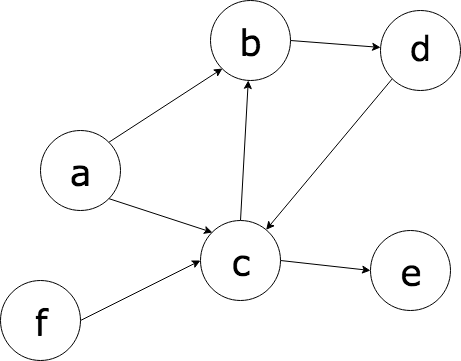
\includegraphics[width=0.4\textwidth]{picstcc/graph.png}
  \caption{Exemplo de grafo $G$. $V(G) = \{a,b,c,d,e,f\}$ e $E(G) =\{ab, ac, cb, bd, dc, fc, ce\}$.}
  \label{graph}
\end{figure}

Um problema genérico de busca em grafo pode ser postulado como ``encontrar o conjunto $C$ de vértices que podem ser alcançados a partir de um vértice $v$'' (alcançar, no caso, refere-se a percorrer os vértices usando os arcos). O conjunto $C$ é chamado \textit{território} de $v$. Assim, para $v = a$ no grafo em \ref{graph}, temos $C = \{ a, b, c, d, e\}$, pois $a$ não alcança apenas o vértice $f$. Podemos adicionar algumas especificações para o problema, como por exemplo encontrar os \textit{caminhos simples}\footnote{Um caminho é uma sequência alternante de vérices e arcos em que cada arco tem pontas nos vértices anterior e posterior na sequência, respectivamente. Um caminho simples é um caminho que não contém \textit{laços}, ou seja, não visita um vértice mais de uma vez.} para os vértices no território de um vértice $v$ (por exemplo, para o território de $c$ em \ref{graph}, temos o conjunto de caminhos simples $\mathcal{P} = \{(c), (c,cb,b,bd,d), (c, ce, e)\}$). Outra especificação envolve uma \textit{função-custo}, que atribui um número real c(e) para cada arco $e \in E$. Pode ser interessante, então, encontrar os caminhos \textit{mínimos} de um vértice ao seu território, onde o custo $c(P)$ de um caminho é a soma $\sum_ec(e)$ dos custos de cada um de seus arcos.

\begin{figure}[!h]
  \centering
  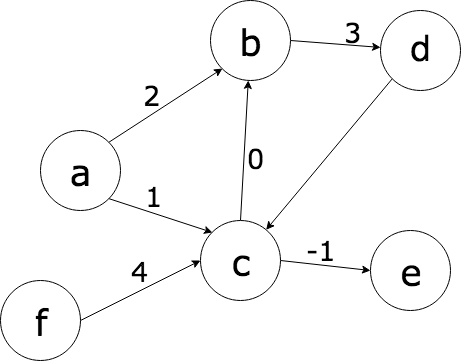
\includegraphics[width=0.4\textwidth]{picstcc/costedgraph.png}
  \caption{Grafo $G$ com uma função-custo $c$ associada. Por exemplo, um caminho mínimo de $a$ a $b$ é $P = (a, ac, c, cb, b)$, onde $c(P) = 1 + 0 = 1.$}
  \label{costedgraph}
\end{figure}

Os dois tipos básicos de algoritmo de busca genérica são a \textbf{busca em largura} (que utiliza \textit{filas} como estrutura de dados) e a \textbf{busca em profundidade} (que, por sua vez, manipula \textit{pilhas}). Ambas fazem uso do conceito de \textit{vizinhos} de um vértice $v$, ou seja, os vértices $w$ tais que exista arco $vw \in E$. Supondo que queiramos encontrar o caminho mínimo de um vértice $v$ até os vértices de um grafo com custos $(V, E, c)$, a \textbf{busca em largura} funciona da seguinte maneira:

\begin{algorithm}
  \caption*{Busca em largura $(V, E, c, v)$:}
  \begin{algorithmic}
    \STATE fila $q \gets \{v\}$
    \STATE custo $c_w \gets \infty, \forall w \in V$
    \STATE caminho $P_w \gets \emptyset, \forall w \in V$
    \STATE \textbf{enquanto} $q \neq \emptyset$:
    \STATE \ind $w \gets $ elemento mais antigo de $q$, remove $w$ da $q$
    \STATE \ind \textbf{para cada} vizinho $u$ de $w$:
    \STATE \ind \ind \textbf{se } o custo até $u$, $c_u > c_w + c_{wu}$:
    \STATE \ind \ind \ind $c_u \gets c_w + c_{wu}$
    \STATE \ind \ind \ind $P_u \gets P_w + (wu, u)$
    \STATE \ind \ind \textbf{se} $u$ não foi expandido \textbf{ então}:
    \STATE \ind \ind \ind marque $u$ como expandido
    \STATE \ind \ind \ind insira $u$ no final de $q$
    \STATE \textbf{devolva} conjunto dos caminhos $P_w, \forall w \in E$
  \end{algorithmic}
\end{algorithm}

Fica como o exercício para o leitor aplicar o algoritmo ao grafo do exemplo \ref{costedgraph}.

\section{Minimax}
\label{sec:minimax}
Nas modelagens de problemas de busca em jogos individuais, normalmente a solução ótima é obtida a partir de uma sequência de ações levando a um estado desejado (que normalmente representa a vitória do agente). Quando o jogo envolve mais de um jogador, é possível que as ações dos outros jogadores influenciem o estado e quais ações podem ser tomadas. Neste caso, chamamos de \textsc{Max} o agente que está querendo maximizar a recompensa final, enquanto o adversário de \textsc{Max} que está tentando fazer com que este não atinja seu objetivo é chamado de \textsc{Min}. O objetivo de \textsc{Max} é, então, encontrar uma estratégia para conseguir a maior recompensa possível, levando em consideração que \textsc{Min} irá sempre tomar a ação que minimiza a recompensa final.

Para exemplificar, vamos supor um jogo trivial representado pela árvore da imagem \ref{minimax} onde \textsc{Max} escolhe uma de três ações alterando o estado inicial, e então \textsc{Min} escolhe uma de três ações alterando o estado obtido pela ação de \textsc{Max}, levando a um estado final com uma recompensa associada.

\begin{figure}[!h]
        \centering
            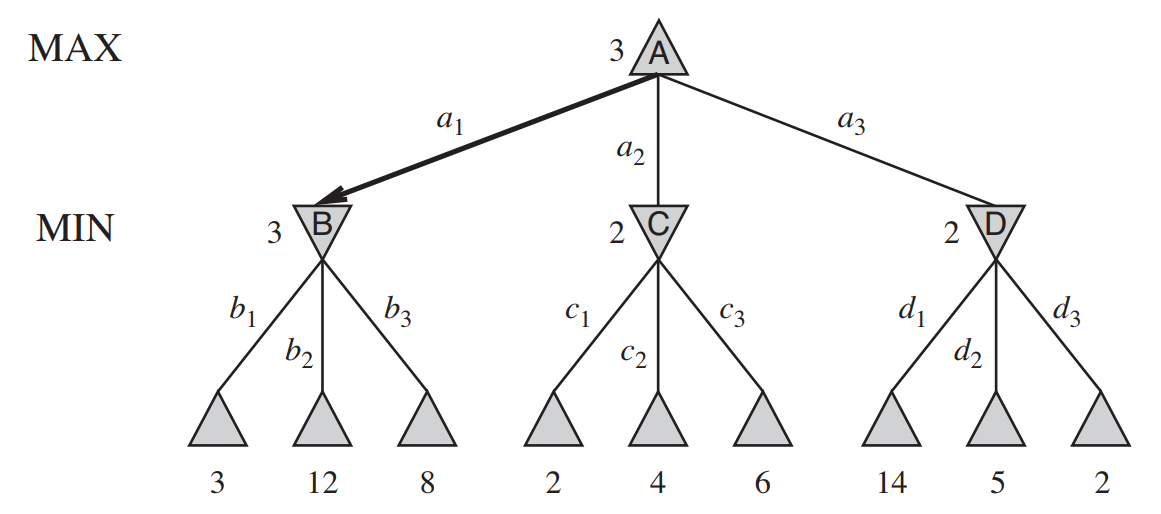
\includegraphics[width=0.9\textwidth]{picstcc/minimax.png}
            \caption{O jogo trivial com as ações possíveis de MAX e MIN. Fonte: \cite[p. 164]{livro}}
            \label{minimax}
\end{figure}

Dada a árvore de jogo, a estratégia ótima pode ser determinada pelo \textbf{valor minimax} de cada nó, que escreveremos como $Minimax(n)$. O valor minimax de um nó é a utilidade, do ponto de vista de MAX, de estar no estado correspondente, assumindo que ambos os jogadores joguem otimamente. Dada uma escolha, MAX prefere mover para um estado de valor máximo, enquanto MIN prefere mover para um estado de valor mínimo:
\begin{equation*}
  Minimax(s) = \\
  \begin{cases} Utilidade(s), &\textrm{se s é um estado terminal}\\
                \max\limits_{a\in A(s)}Minimax(T(s,a)), &\textrm{se o jogador é MAX}\\
                \min\limits_{a\in A(s)}Minimax(T(s,a)), &\textrm{se o jogador é MIN}\\
  \end{cases}
\end{equation*}
onde $A(s)$ é uma função que devolve as ações possíveis a partir de um estado $s$, e $T(s, a)$ é uma função de transição que devolve o estado resultante de se tomar a ação $a$ a partir do estado $s$.

Aplicando as definições acima na figura \ref{minimax}, os nós no nível mais baixo da árvore recebem seu valor a partir da função de $Utilidade$ do jogo. O primeiro nó de MIN, rotulado por $B$, tem três estados sucessores com valores 3, 12 e 8, então seu valor minimax é 3. Podemos também identificar a \textbf{decisão minimax} a partir da raiz: a ação $a_1$ é a escolha ótima para \textsc{Max} pois leva ao estado com maior valor minimax.
